\documentclass{beamer}
\usepackage[orientation=portrait,size=a0,scale=1.4,debug]{beamerposter}
\mode<presentation>{\usetheme{ZH}}
\usepackage{chemformula}
\usepackage[utf8]{inputenc}
\usepackage[german, english]{babel} % required for rendering German special characters
\usepackage{siunitx} %pretty measurement unit rendering
\usepackage{hyperref} %enable hyperlink for urls
\usepackage{ragged2e}
\usepackage[font=scriptsize,justification=justified]{caption}
\usepackage{array,booktabs,tabularx}
\usepackage[ruled]{algorithm2e}
\usepackage{algorithmic}
\usepackage{bbm}

\newtheorem*{remark}{Remark}

\newcommand{\R}{{\mathbb{R}}}
\newcommand{\E}{{\mathbb{E}}}
\newcommand{\bbP}{{\mathbb{P}}}
\newcommand{\bbI}{{\mathbbm{1}}}

\newcolumntype{Z}{>{\centering\arraybackslash}X} % centered tabularx columns
% \sisetup{per=frac,fraction=sfrac}

\title{\huge Optimal Transport for Super Resolution Applied to Astronomy Imaging}
\author{Michael G. Rawson$^{1,2}$, Jakob Hultgren$^2$}
\institute{$^{1}$ Pacific Northwest National Laboratory, Seattle, WA, USA \\ 
$^{2}$ University of Maryland at College Park, College Park, MD, USA
}
\date{\today}

% edit this depending on how tall your header is. We should make this scaling automatic :-/
\newlength{\columnheight}
\setlength{\columnheight}{104cm}

\begin{document}
\begin{frame}
\begin{columns}
	\begin{column}{.5\textwidth}
		\begin{beamercolorbox}[center]{postercolumn}
			\begin{minipage}{.98\textwidth}  % tweaks the width, makes a new \textwidth
				\parbox[t][\columnheight]{\textwidth}{ % must be some better way to set the the height, width and textwidth simultaneously
					\begin{myblock}{Super Resolution}
Super resolution seeks to improve image resolution without further data collection.
This is possible, given constraints that give a well-posed inverse problem, for example smoothness or \textbf{sparsity}.
\begin{figure}
\centering\includegraphics[width=.7\textwidth]{img/Super_resolution.jpg}
\end{figure}
					\end{myblock}\vfill
					\begin{myblock}{Optimal Transport}
    Let $\mu\in\mathbb R^n_{\ge 0}, \nu \in \mathbb R^m_{\ge 0}$ be probability vectors and $C\in \mathbb R^n\times \mathbb R^m$. Then the optimal transport plan from $\mu$ to $\nu$ is                            
\begin{equation} 
    \arg\min_{P\in \Pi(\mu,\nu)} \sum_{i=1}^n \sum_{j=1}^n C_{ij} P_{ij} 
\end{equation}
where 
$ \Pi(\mu,\nu) = \{P\in\mathbb R^{n\times m}: \sum_{i=1}^n P_{ij} = \nu_j\ \forall j, \sum_{j=1}^n P_{ij} = \mu_i\ \forall i\}. $
					\end{myblock}\vfill
					\begin{myblock}{Wasserstein Inverse Problem for Super Resolution}
    For a measurement $\nu$ and positive regularization parameter $\lambda$, we define the \emph{sparse approximation} of $\nu$ as a minimizer 
\begin{equation}
    \mu_* = \arg\min_{\mu \in \bbP(X)} d_W^\epsilon(\mu,\nu) + \lambda H(\mu).
    \label{eq:sparseNeigh}
\end{equation}
At least one minimizer exists by compactness of the finite dimensional probability simplex. The entropy term favors sparse solutions. There is a trade-off between sparsity of the solution and proximity to the measurement. 
					\end{myblock}\vfill
% 					\begin{myblock}{Entropy}
%     For a probability mass function $p:\mathcal J\rightarrow \mathbb R$ (non-negative and sums to 1), we will use $H(p)$ to denote its entropy,
% \begin{equation} 
%     H(p) = -\sum_{\iota \in \mathcal J} p(\iota) \ln(p(\iota)) \label{eq:Entropy}. 
% \end{equation}

%     \textbf{Key point:} Sparse arrays have low entropy. 
% 					\end{myblock}\vfill
% 					\begin{myblock}{Entropic regularization of Optimal Transport}
%     Approximate optimal transport distances can be computed by solving the entropic regularization of optimal transport
%     $$ \arg\min_{P\in \Pi(\mu,\nu)} \sum_{i=1}^n \sum_{j=1}^n C_{ij}P_{ij} - \epsilon H(P). $$
    
%     This is equivalent to the matrix scaling problem, more precisely finding positive multipliers $f\in \mathbb R^n, g\in \mathbb R^m$ such that the matrix
%     $$ (f_i e^{-C_{ij}/\epsilon} g_j) \in \Pi(\mu,\nu). $$

% 					\end{myblock}\vfill
    					\begin{myblock}{Theoretic Results}

\begin{theorem}[\cite{rawson_astro}]
Let $\nu = \frac{1}{k}\sum_{i=1}^k \delta_{p_i}$ where $p_i\in \mathbb R^d$ and $\tilde\nu$ be the noisy signal acquired by sampling, for each $i$, $n$ points according to a normal distribution centered at $p_i$ with independent components of variance $\sigma^2$. Then the Wasserstein distance between $\nu$ and $\bar\nu$ is bounded by a random variable with expected value $d\sigma^2$ and variance $2d\sigma^4/N$,  where $N=nk$ is the total number of points sampled.  
\end{theorem}

\begin{theorem}[\cite{rawson_astro}]
    \label{thm1}
    Assume $\nu$ is a sparse signal and $\bar\nu$ is a noisy signal such that 
    $d_w(\nu,\bar\nu) < \delta $. Then the solution of 
    \begin{equation*} \label{eq:dualConstraint} 
        \mu=\arg\min_{\mu : d_W(\bar\nu,\mu) \le \delta} H(\mu) 
    \end{equation*} 
    will identify the structure of $\mu$, i.e. have the same support as $\mu$, if $||\nu||_0 \leq ||\mu||_0$ for all $\mu$ such that $d_W(\mu,\bar\nu)<2\delta$, with equality only if $\mu$ and $\nu$ has the same support.  
\end{theorem}

\begin{remark}
    \quad The conditions in Theorem~\ref{thm1} can be summarized as a low enough noise level $\delta$ and enough sparsity of the true signal $\nu$ (making it a local minimizer of the $L^0$-norm). It is interesting to note that these conditions are essentially necessary: if the inequality in Theorem~\ref{thm1} is violated by some $\mu$ closer than $\delta$ to $\bar\nu$, then the solution of \eqref{eq:dualConstraint} does not identify the structure of $\nu$. 

    \quad Noise is high entropy, hence it is expected that the noise can be removed by minimizing the entropy. However, if the signal-to-noise ratio is too low, this reconstruction is underdetermined.
\end{remark}

\begin{theorem}[\cite{rawson_astro}]
    Fix a positive probability vector $\nu\in\R^d_{>0}$ such that all elements of $\nu$ are distinct. 
    Then the sparse recovery is continuous to perturbations around $\nu$ for small $\lambda$, i.e. for every $\epsilon'>0$ there exists $\delta>0$, such that 
    if $d_W(\nu,\nu')<\delta$,
    $\mu_* = \arg\min_{\mu \in \bbP(X) : d_W(\mu, \nu)<\lambda} H(\mu)$,
    and 
    $\mu_*' = \arg\min_{\mu \in \bbP(X) : d_W(\mu, \nu')<\lambda} H(\mu)$
    then $\|\mu_*-\mu_*'\| < \epsilon'.$
    \label{thm:robust}
\end{theorem}

					\end{myblock}\vfill
     
		}\end{minipage}\end{beamercolorbox}
	\end{column}
	\begin{column}{.5\textwidth}
		\begin{beamercolorbox}[center]{postercolumn}
			\begin{minipage}{.98\textwidth} % tweaks the width, makes a new \textwidth
				\parbox[t][\columnheight]{\textwidth}{ % must be some better way to set the the height, width and textwidth simultaneously

					\begin{myblock}{Method}
% \begin{algorithm}[H]
% \textbf{Input:} 

% $\mu, \nu \in \R^n$ : positive probability vectors,

% $C\in\R^{n \times n}$ : cost matrix,

% $\epsilon$ : positive regularization parameter

% \textbf{Output:}

% $d_W^\epsilon \in \R$ : regularized distance between $\mu$ and $\nu$,

% $F \in \R^n$ : gradient of $d_W^\epsilon(\mu,\nu)$ with resp. to $\mu$ at $\mu$,

% $G \in \R^n$ : gradient of $d_W^\epsilon(\mu,\nu)$ with resp. to $\nu$ at $\nu$
    
%     \textbf{Begin:} 

%     $f = (1,\ldots,1)\in \R^n$
    
%     $g = (1,\ldots,1)\in \R^n$
    
% 	\While{$f$ and $g$ have not converged}
%  	{
%  	    \For{$1 \le i \le n$}{
%      	$f_i = \mu_i / \left(\sum_j \exp(-C_{ij}/\epsilon) g_j\right)$ 
%      	}
%      	\For{$1 \le j \le n$}{
%      	$g_j = \nu_j / \left(\sum_i \exp(-C_{ij}/\epsilon) f_i\right)$ 
%      	}
%   	}
  	
%     $d_W^\epsilon = \sum_{i=1}^n \sum_{j=1}^n f_i g_j \exp(-C_{ij} /\epsilon) C_{ij}$ 
  	
%   	$F = -\epsilon \ln(f)$
  	
%   	$G = -\epsilon \ln(g)$\\
  	
% 	\caption{ The Sinkhorn Algorithm for Optimal Transport Distances}
% \end{algorithm}

\begin{algorithm}[H]
    \textbf{Input:} 

$X \in \R^{N \times m \times m}$ : $N$ images size $m \times m$,

$\lambda \in \R$ : positive noise level,

$0 < \epsilon < 1$ : optimal transportation regularization,

$C\in\R^{m^2 \times m^2}$ : cost matrix,

$ J_{\lambda,\epsilon}(x,v) := d_W^\epsilon(x,v) + \lambda H(v) $

    \textbf{Output:}

$K \in \R^N$ : star cluster classification
    
    \textbf{Begin:}
    
    $K = 0$
    
	\For{$i=1,2,...,N$}
 	{
% $ V_i = \arg\min_{v} d_W^\epsilon(X_n,v) + \lambda H(v)$\\
        $ v = X_i $ \\
    	\While{ $v$ has not converged }
 	    {
$w = \nabla d_W^\epsilon(X_i,\cdot)|_v + \lambda \nabla H|_v $ \\
$ w = w - \langle w, \frac{1}{m} \bbI \rangle \cdot \frac{1}{m} \bbI $ \\
$ \alpha = \sup\{\alpha \in \R : J_{\lambda,\epsilon}(v) > J_{\lambda,\epsilon}(v - \alpha w) \}$ \\
            $ \alpha = \min\{0.01, \alpha\}$\\
 	        $ v = v - \alpha w $;
 	        $ v = diag(\bbI_{v > 0}) \ v $;
 	        $ v = v/\|v\|_1 $
 	    }
 	    $V_i = v$;
     	$\delta = \max V_i$
     	
        \If{ $rank(H_0(V_i^{-1}([0.75 \delta,\ \delta]))) == 1$ }{ 
            $ K_i = 1 $ 
        }
  	}
	\caption{ O.T. Super Resolution Clustering \cite{rawson_astro}}
\end{algorithm}

					\end{myblock}\vfill

					\begin{myblock}{Example}
                        Let measurement $ \hat\nu = (0.2, 0.15, 0, 0, 0, 0.1, 0.15, 0.2, 0.15, 0.1) $. 
                        \begin{figure}
                        \centering
        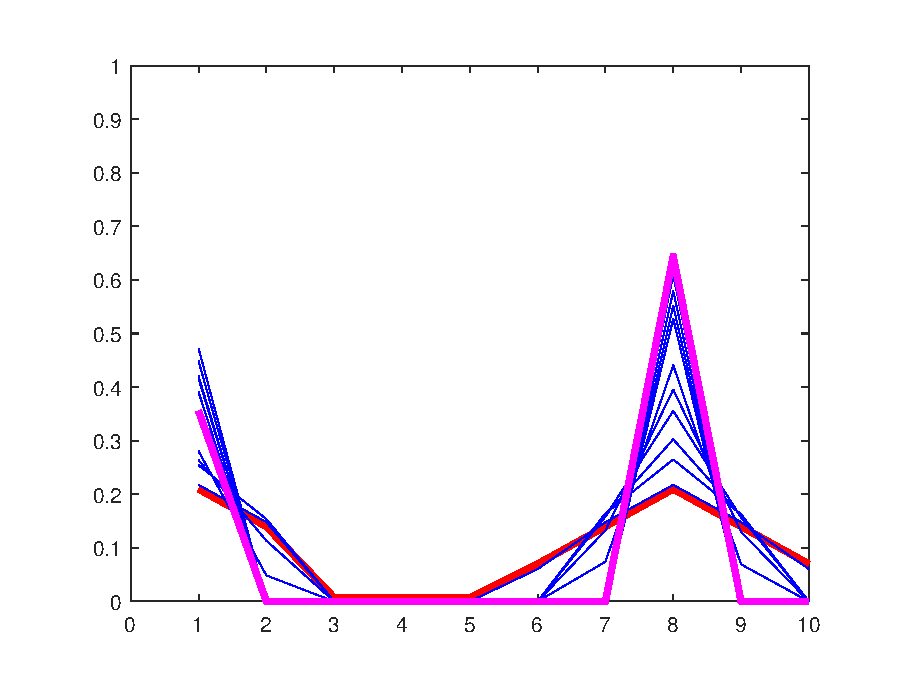
\includegraphics[width=.6\textwidth]{img/OT_gradient_descent_1D_lambda=10.eps}
                        \end{figure}
                        
                        Plot of super resolution O.T. method. Red line is initial distribution. Blue lines are steps along gradient. Pink line is final, converged distribution.

                        Sparsity level $\lambda=10$. Solution $ \nu = (0.35,0,0,0,0,0,0,0.65,0,0)$. 

					\end{myblock}\vfill
     \begin{myblock}{Star Clustering Application}
\begin{itemize}
    \item The formation and evolution of star clusters\cite{perez}
    \item Algorithmically detect star clusters in images of sky patches
    \item State of the art method trains a convolutional neural network (CNN) to classify each region in an image as containing a star cluster or not \cite{perez}
    \item Neural networks are notoriously computationally expensive, sensitive to noise, and inflexible to appending or removing data variables
\end{itemize}

Confusion matrix of O.T. method on LEGUS data compared to StarcNet \cite{perez}. Column gives StarcNet classification and row gives O.T. classification \cite{rawson_astro}:

\begin{table}
\begin{center}
\begin{tabular}{c|c|c|}
 & StarcNet Cluster & StarcNet Not Cluster \\
\hline
O.T. Cluster     & 25\% (32) & 13.3\% (17)  \\
\hline
O.T. Not Cluster & 12.5\% (16) & 49.2\% (63)  \\
\hline
\end{tabular}
\label{table:2}
\end{center}
\end{table}

     \end{myblock}\vfill
					\begin{myblock}{References}
						\footnotesize
						\bibliographystyle{abbrv}
						\bibliography{ref.bib}
					\end{myblock}\vfill
		}\end{minipage}\end{beamercolorbox}
	\end{column}
\end{columns}
\end{frame}
\end{document}

